\section*{Related work}\label{ch:ch2label}

\subsection*{Physically based differentiable rendering}

Until now, the reseachers have been focusing on differentiable light transport integral.
These include solving geometric discontinuity problem on the integral\cite{li2018differentiable, loubet2019reparameterizing, zhang2020path}. In all these works, the derivatives with respect to scene parameters are calculated by automatic differentiation. Especially, by reverse-mode differentiation the derivatives with respect to multiple scene parameters are computed at once. Though multi-derivatives are possible, we need another technique about some parameters or joint optimization problem, due to the local minima.

\subsection*{Laplacian smooth gradient descent}

Stochastic gradient descent (SGD) is the workhorse in modern optimization technique. However, due to the variance, shows somtimes the result cannot overcome local stucking. 

Osher et al\cite{osher2018laplacian} suggested the method to take larger steps than SGD, which is enabled by simply multiplicating gradient with discrete one-dimensional laplacian.

\subsection*{Laplacian smoothing in computer graphics}

In geometry processing, the laplacian operator has been the key tool for solving many kind of geometry problem. Though there may be many references about many laplacian properties, discrete laplacians are enough in here.

\begin{figure}
    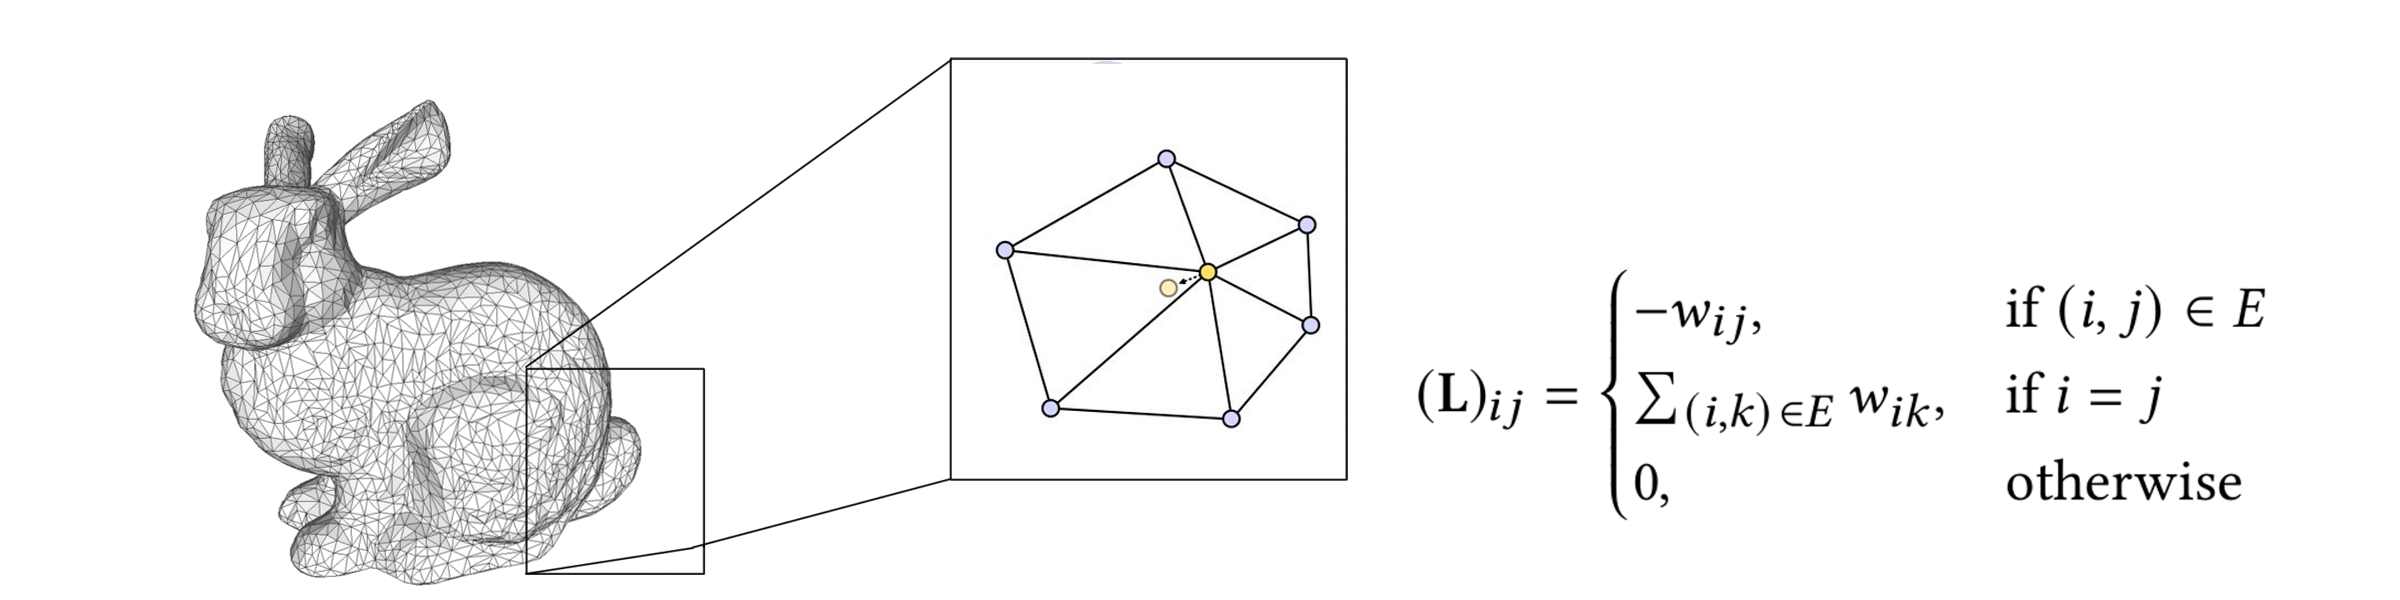
\includegraphics[width=\textwidth]{figures/related-work-1.png}
    \caption{Discrete Laplaican on Mesh}
    \label{fig:discretelaplacian}
\end{figure}

% TODO
Discrete laplacian\ref{fig:discretelaplacian} some depiction
Generally, cotangent matrix, in real combination, 
this is combined with mesh massmatrix 

Nicolet et al\cite{Nicolet2021Large} shows the application method of laplacian smooth to mesh optimizing on differentiable rendering. This works improve the convergence speed and the quality of optimization result.

The authors convert the iterative update form in gradient descent like below:
\begin{align}{\label{eq1}}
	x \leftarrow x - \gamma (I + \lambda L)^{-p} 
\end{align}
In here, the $L$ is calculated from discrete laplacian on mesh.

This form can be interpreted as various meaning. As mentioned before, 
also, in differentiable rendering, in the 
we can think as laplacian smooth gradient using mesh propertices. 
Quasi-Newton's method for gradient descent using the mesh properties

From the point of view of geometry processing,
Or, on each iteration, filtering noisy vertices from the target mesh before gradient descent step.







